    \chapter{Methodology}
       \section{SOFTWARE DEVELOPMENT APPROACH}
       Agile development is a software development approach that emphasizes incremental progress and rapid cycles. It involves releasing small increments of functionality that build upon previous versions. Thorough testing is conducted for each release to ensure software quality. Agile is often employed for time-critical applications. Although this project is not time-critical this model seems to be the most optimal and practical in our case.
       \begin{figure}[hbt!]
           \center{
               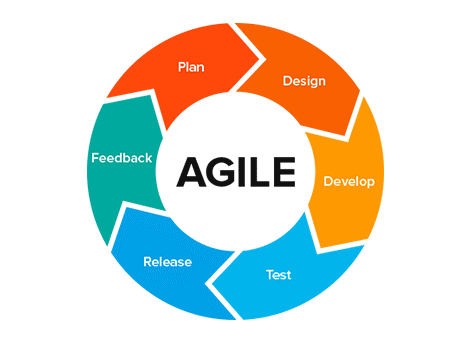
\includegraphics[width=0.75\textwidth]{./img/agile.png}
               \caption{Agile Model for Software Development}
               \subcaption*{\textit{source: \textcolor{blue}{https://mobilelive.medium.com/agile-development-a-comprehensive-guide-for-the-modern-era-d2fe9ae7b395}}}
           }
       \end{figure}
       
       \section{Implementation}

       \subsection{Data Collection}
       Datas of Nepali Text will be collected from different nepali news and governmental websites for training.
       
    %    \subsection{Data Preprocessing}
    %    \subsubsection{Normalization}
    %    In English, we have uppercase and lowercase letters that sound the same when we speak them. Similarly, in Nepali, there are different ways to write certain vowel sounds that sound the same when spoken. For example, the words 
    % %    नेपाली and नेपालि     
    %     are pronounced the same way, but they are written differently. This can cause confusion and mistakes in written Nepali, making the data messy. Normalization is the process of finding these differences and making sure they are all written in the same way to clean up the data.

        \subsection{Transformers}
        A transformer model is a neural network that learns context and thus meaning by tracking relationships in sequential data like the words in this sentence.
        Transformer models apply an evolving set of mathematical techniques, called attention or self-attention, to detect subtle ways even distant data elements in a series influence and depend on each other.
        First described in a 2017 paper from Google\cite{vaswani2023attention}, transformers are among the newest and one of the most powerful classes of models invented to date. They’re driving a wave of advances in machine learning some have dubbed transformer AI.
        Stanford researchers called transformers “foundation models” in an August 2021 paper\cite{bommasani2021opportunities} because they see them driving a paradigm shift in AI. The “sheer scale and scope of foundation models over the last few years have stretched our imagination of what is possible,” they wrote.


        \newpage
        \begin{figure}[hbt!]
            \center{
                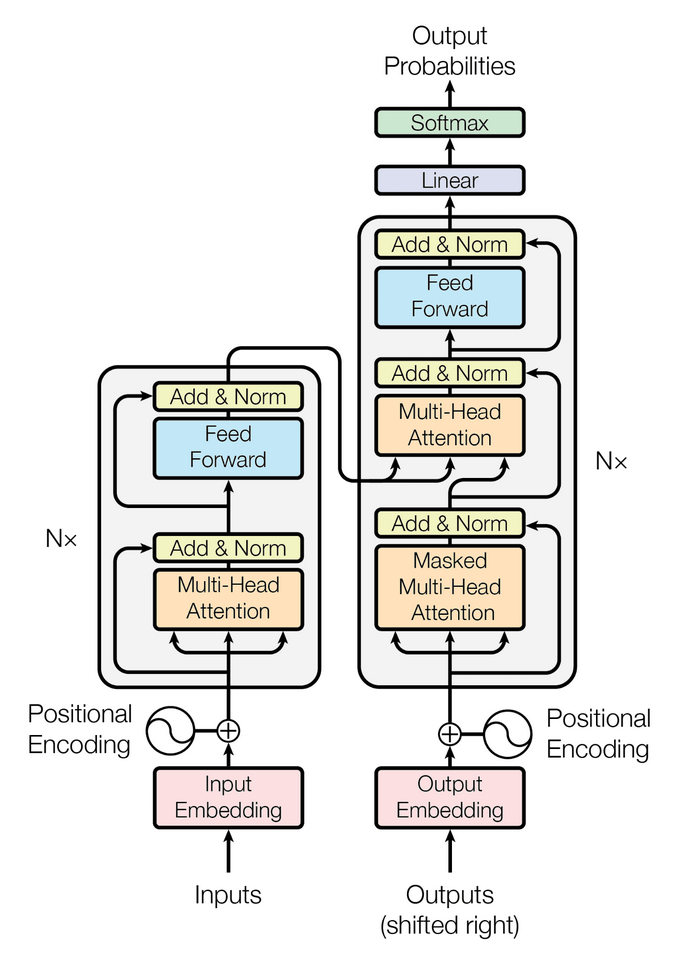
\includegraphics[width=0.80\textwidth]{./img/attention_research_1.png}
                \caption{The Transformer - model architecture.\cite{vaswani2023attention}}
                }
        \end{figure}

        \newpage
        \subsection{BERT}
        BERT stands for Bidirectional Encoder Representations from Transformers. It is designed to train deep bidirectional representations from unlabeled text by jointly conditioning on both left and right context.
        % As a result, the pre-trained BERT model can be fine-tuned with just one additional output layer to create state-of-the-art models for a wide range of NLP tasks.


        \newpage
        \subsection{Proposed System}
        \begin{figure}[hbt!]
            \center{
                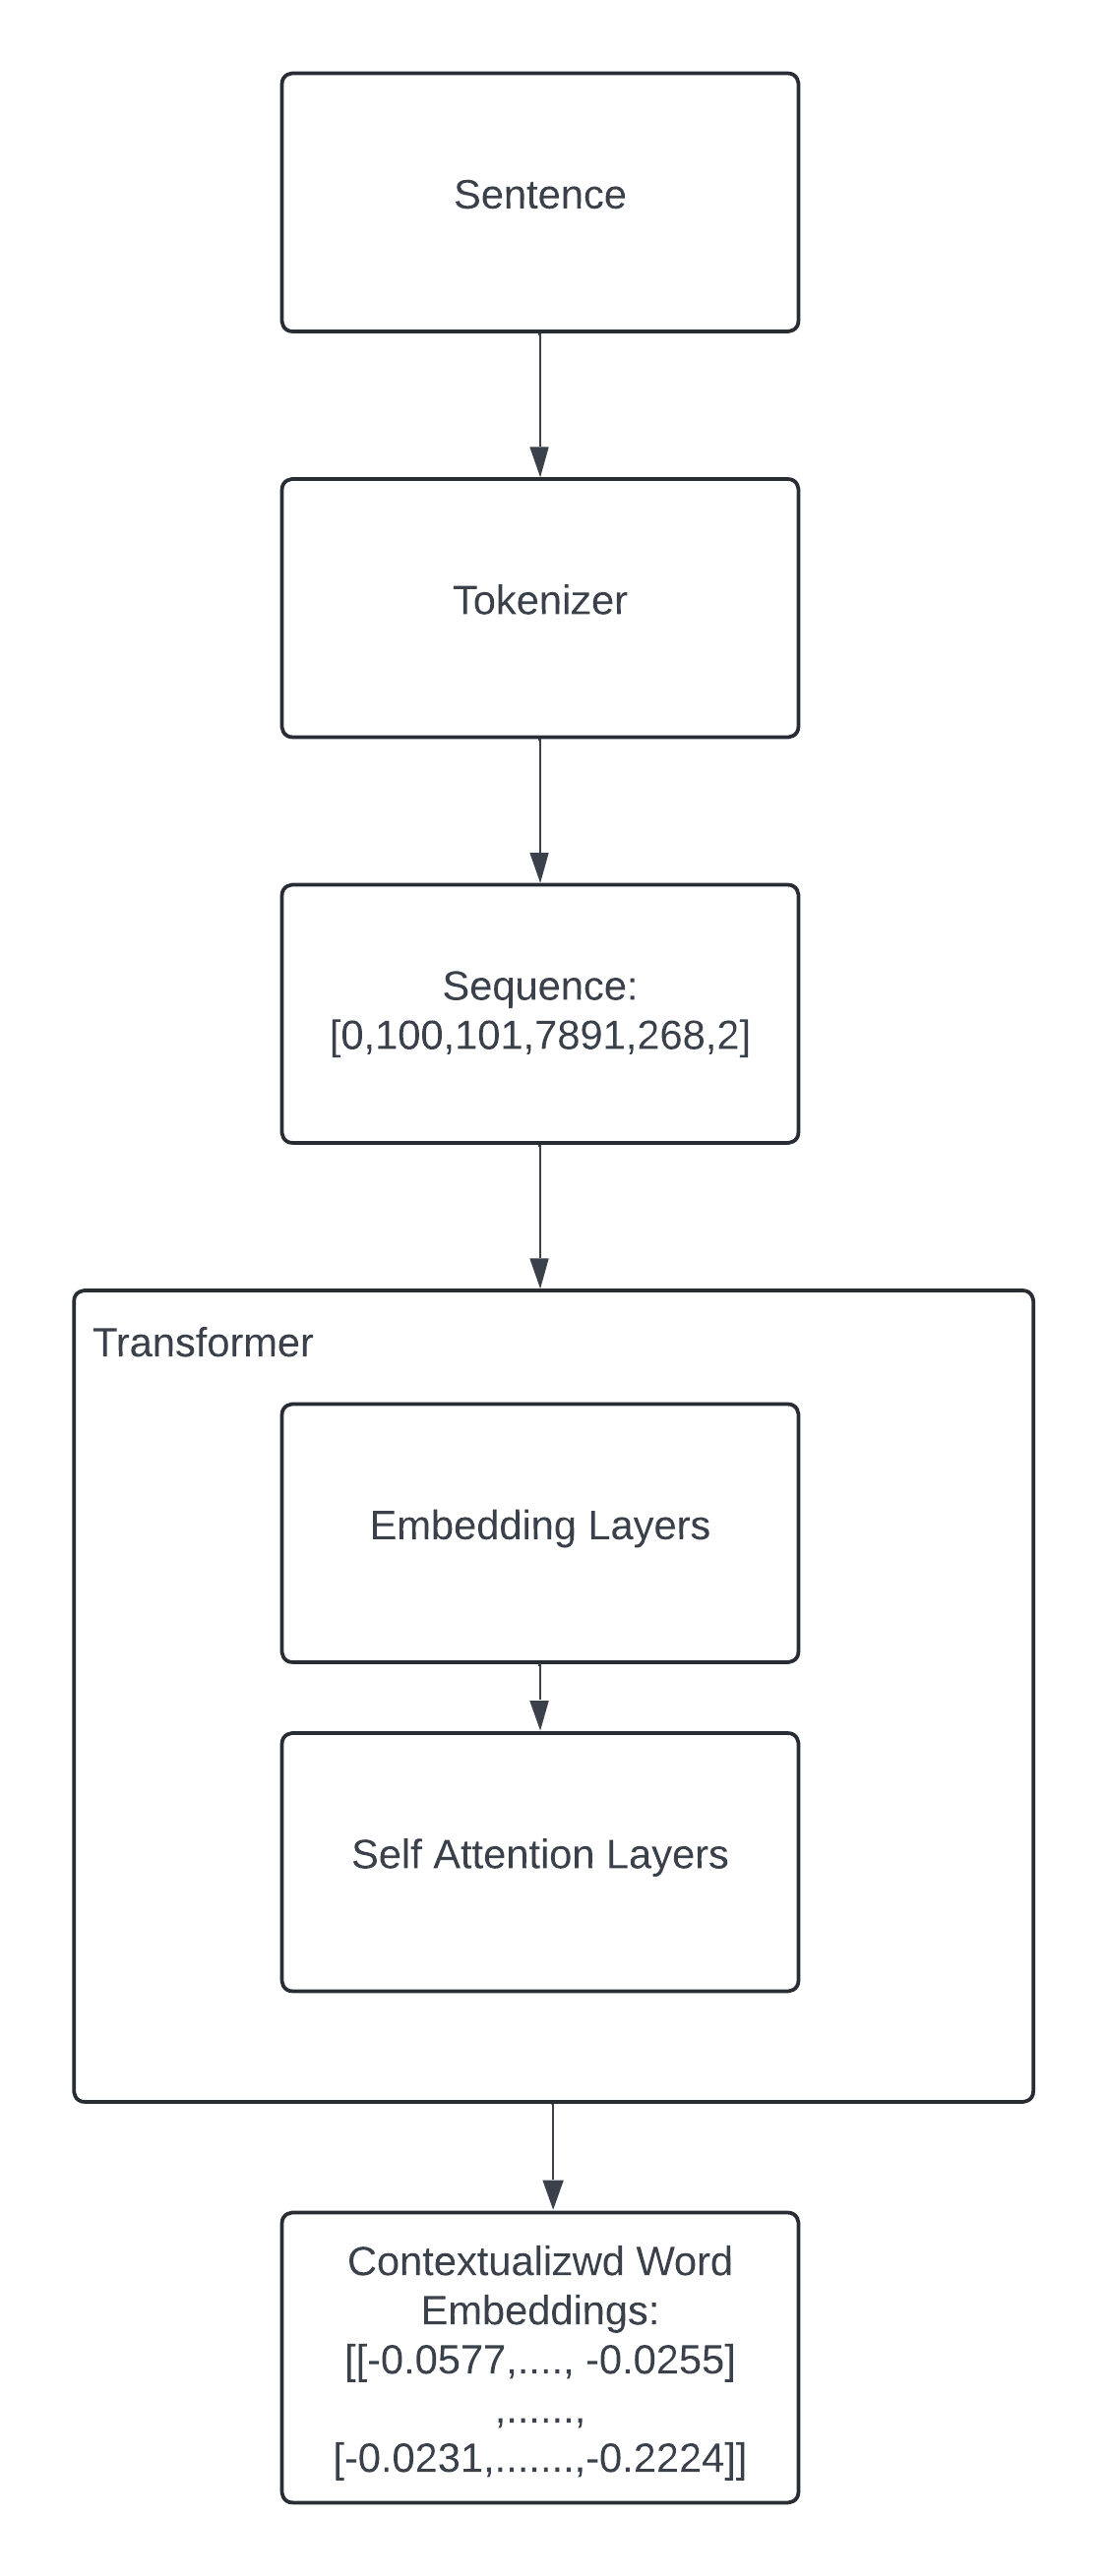
\includegraphics[width=0.55\textwidth]{./img/Block_Diagram.png}
                \caption{Block diagram of Proposed Sytem}
                }
        \end{figure}
       
        \newpage
        % \justifying 
        \subsection{Gantt Chart}
        \vspace{2em}
        \begin{figure}[htbp]
            \hspace*{-1cm} % Adjust the value as needed
            \begin{ganttchart}[
                hgrid,
                vgrid,
                x unit=2em,
                y unit chart=3em,
                time slot format=isodate-yearmonth,
                time slot unit=month,
                title height=1,
                bar/.append style={fill=blue!40},
                bar height=0.7,
                bar label node/.append style={align=right, text width=7em},
                group height=0.6,
                group peaks height=0.2,
                group peaks tip position=0,
                group/.append style={draw=black, fill=green!50},
                group label font=\small
                ]{2024-04}{2025-03}
                \gantttitlecalendar{year} \\
                \gantttitlecalendar{month} \\
                \ganttbar{Requirement Analysis}{2024-04}{2024-05} \\
                \ganttbar{Feasibility Study}{2024-04}{2024-05} \\
                \ganttbar{Software Design}{2024-05}{2024-06} \\
                \ganttbar{Implementation}{2024-06}{2025-01} \\
                \ganttbar{Testing}{2025-01}{2025-02} \\
                \ganttbar{Research}{2024-04}{2025-01}\\
                \ganttbar{Documentation}{2024-04}{2025-03}\\
            \end{ganttchart}
            \caption{Gantt Chart}
        \end{figure}